\documentclass[11pt,a4paper]{article}
\usepackage[utf8]{inputenc}
\usepackage[T1]{fontenc}
\usepackage{amsfonts}
\usepackage[french]{babel}
\frenchbsetup{StandardLists=true} % à inclure si on utilise \usepackage[francais]{babel}
\usepackage{enumitem}
\usepackage{amssymb}
\usepackage{amsmath}
\usepackage[left=2cm,right=2cm,top=2cm,bottom=2cm]{geometry}
\usepackage{multirow}
\usepackage[dvipsnames]{xcolor}

\usepackage[T1]{fontenc}
\usepackage{fouriernc}
\usepackage{graphicx}
\usepackage{tikz-osci}

\usepackage{setspace}
\singlespacing

\usepackage{pstricks}

\usepackage[
  european resistor,
  RPvoltages,
  european current,
  european voltage,
  straightvoltages
  ]{circuitikz}
\usepackage{xkeyval}
\usepackage{pst-labo}


\usepackage{multicol}
\usepackage{caption}
\usepackage{fancyhdr}
\pagestyle{fancy}
\renewcommand\headrulewidth{1pt}
\fancyhead[L]{Lycée Denis Diderot }
\fancyhead[R]{Classe de 1 Bac Pro }
\setcounter{page}{1}\fancyfoot[C]{page \thepage}
\fancyfoot[R]{Année 2024-2025}
\fancyfoot[L]{Alexis RUIZ}
\usepackage{multirow,tabularx,booktabs}
\usepackage[tikz]{bclogo} 

\newcommand{\cadreblanc}[1]{%
\medskip\framebox[\linewidth][c]{%
\rule{0mm}{#1mm}}\par
\medskip}

\usepackage{awesomebox}
\setlength{\aweboxvskip}{0mm}
\usepackage{pifont}
\usepackage{chemmacros}
\chemsetup{modules=all}
\setlength{\columnseprule}{.25mm}

\renewcommand{\arraystretch}{2.5}
\newcommand*\acocher{\quitvmode{\fboxsep0pt \fboxrule0.8pt \fbox{\vrule height1.8ex depth.1ex width0pt \vrule height0pt depth0pt width1.9ex }}}

\newcolumntype{C}[1]{>{\centering\arraybackslash }b{#1}}

\newcommand{\code}{\awesomebox[black]{2pt}{

\includegraphics[scale=0.15]{../Chapitre 1 - Energie et puissance électrique/images/frame.png}
}{black}}

\newcommand{\moteur}{\awesomebox[black]{2pt}{

\includegraphics[scale=1]{images/moteur.jpg} 
}{black}}

\newcommand{\defconclusion}{\awesomebox[black]{2pt}{\rotatebox{90}{\Large{\textbf{Conclusion}}}}{black}}

\newcommand{\defbox}{\awesomebox[black]{2pt}{
\includegraphics[scale=0.5]{../Chapitre 1 - Energie et puissance électrique/images/appel exam.png}}{black}}

  \newenvironment{itemize*}%  % listes compactes
    {\begin{itemize}%
      \setlength{\itemsep}{0pt}%
      \setlength{\parskip}{0pt}}%
    {\end{itemize}}

\frenchbsetup{StandardLists=true}

\newcommand{\ecranoscillo}{
\begin{tikzpicture}[
  scale=0.7,
  screen/.style={white!50!,draw=black,thick},
  trace/.style={black, ultra thick},
  axes/.style={thick}]

  \begin{scope}[xshift=7cm,yshift=8cm,samples=150]
    \fill[white,rounded corners=0.3cm,draw=black,thick](-5.5,-4.5)
      rectangle (5.5,4.5);
    \fill[screen] (-5.0,-4.0) rectangle (5.0,4.0);
    
    %\draw[trace,red] plot(\x,{1.8*sin((1.6*\x) r)}); % r for radians...
    
    %\draw[trace] plot(\x,{-1+1.25*sin((0.75*\x) r});
    
    \draw[thin] (-5.0,-4.0) grid (5.0,4.0);
    \draw[axes] (-5,0)--(5,0); % Time axis
    \draw[axes] (0,-4)--(0,4);
    \foreach \i in {-4.8,-4.6,...,4.8} \draw (\i,-0.1)--(\i,0.1);
    \foreach \i in {-3.8,-3.6,...,3.8} \draw (-0.1,\i)--(0.1,\i);
\end{scope}
\end{tikzpicture}
}



\begin{document}

\flushleft \textbf{NOM : \hfill Classe : \hspace{3cm} ~~\\[2mm]
Prénom:\\[0,4cm]
}
\hrule\
\\[0,2cm]

\begin{center}
 \LARGE{TP2  - Mesure du déphasage du à une bobine}
\end{center}

\vspace{3 mm}

\normalsize

\hrule\
\\[0,2cm]
   \begin{center}
   \textbf{Le soin et la rédaction interviendront dans la notation.}
   \end{center} 

\fcolorbox{black}{white!30}{\textbf{Introduction}}
\begin{multicols}{2}
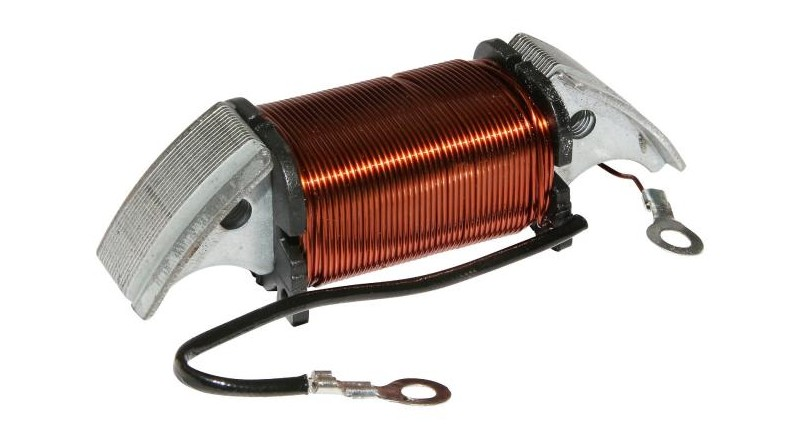
\includegraphics[scale=0.32]{images/bobine-allumage-basse-tension-interieur-ciao-px.jpg}

\columnbreak

Dans l’industrie, un grand nombre de systèmes sont
constitués de circuits inductifs. \\ On les retrouve dans les
moteurs, les générateurs et les transformateurs. Ils
sont également utilisés dans des circuits où ils
réalisent des fonctions plus compliquées.


\end{multicols}

\vfill 
\dotfill 
\vfill

\fcolorbox{black}{white!30}{\textbf{Activité 1 : }}

La tension et l'intensité dans un circuit électrique peuvent être modélisées par deux courbes sinusoïdales de même période $T$./ Deux cas sont possibles : 
\begin{itemize}
   \begin{minipage}{.62\textwidth}%
    \item si les extremum sont aux mêmes instants, les deux grandeurs sont en phase. C'est ce que l'on observe pour un circuit composé seulement de résistors (Four, bouilloire, appareil à raclette ...)
    \end{minipage}%
    \hfill
    \begin{minipage}{.30\textwidth}%
\osci[%
scale=0.48,
second channel=1, %1 pour activer la deuxième voie, 0 sinon.
screen offset one=0, %Décalage vertical de la voie 1 sur l’écran
screen offset two=0, %Décalage vertical de la voie 2 sur l’écran
time div=5, %Durée par division (en ms)
voltage div one=5, %Tension par division (en V) pour la voie 1
voltage div two=2, %Tension par division (en V) pour la voie 2
sample rate=200, %Taux d’échantillonnage
xy mode=0, %1 pour l’activer, 0 sinon 
func one=12*sin(2*180/0.020*x),
func two=3*sin(2*180/0.020*x), 
color one=000000, %Couleur de la voie 1 (en hexadecimal)
color two=808080, %Couleur de la voie 2 (en hexadecimal)
graph back color=FFFFFF,
info back color=D6D6D6,
info text color=000000,
main axis color=000000,
grid color=CCCCCC
]


    %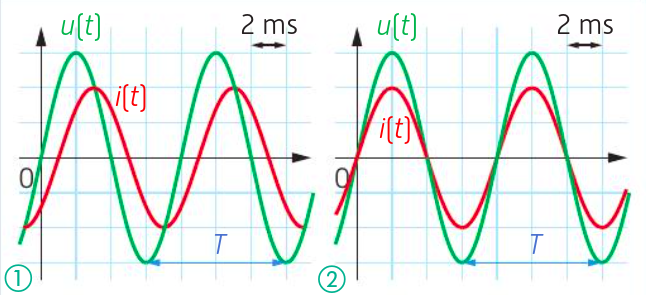
\includegraphics[width=\textwidth]{images/Activite.png}
    \end{minipage}%
    
    
    \item si les courbes sont décalées d'une durée $\Delta t$ (en $s$), elles sont déphasées d'un angle $\varphi$ (en radian ou en degrés) avec : 
    \large{
    $$\varphi = 2\pi\times \dfrac {\Delta  t}{T} \mathrm{~~en~radians} = 360 \times \dfrac {\Delta  t}{T} \mathrm{~~en~degrés}$$}
    \normalsize
    C'est ce que l'on observe pour un circuit contenant une bobine (moteurs, plaques à induction ...) \\[3mm]
    
    \begin{minipage}{.52\textwidth}%
    \begin{enumerate}
        \item Déterminez l'écart de temps $\Delta t $ (en s) entre les deux courbes : \\[2mm]
        \cadreblanc{10}
        \item Calculer, en degrés, le déphase $\varphi$ (arrondir à l'unité). \\[2mm]
        \cadreblanc{18}
        \end{enumerate}

    \end{minipage}%
\hfill
    \begin{minipage}{.4\textwidth}%


\osci[%
scale=0.68,
second channel=1, %1 pour activer la deuxième voie, 0 sinon.
screen offset one=0, %Décalage vertical de la voie 1 sur l’écran
screen offset two=0, %Décalage vertical de la voie 2 sur l’écran
time div=5, %Durée par division (en ms)
voltage div one=5, %Tension par division (en V) pour la voie 1
voltage div two=2, %Tension par division (en V) pour la voie 2
sample rate=200, %Taux d’échantillonnage
xy mode=0, %1 pour l’activer, 0 sinon 
func one=12*sin(2*180/0.020*x),
func two=3*sin(2*180/0.020*x-90), 
color one=000000, %Couleur de la voie 1 (en hexadecimal)
color two=808080, %Couleur de la voie 2 (en hexadecimal)
graph back color=FFFFFF,
info back color=D6D6D6,
info text color=000000,
main axis color=000000,
grid color=CCCCCC
]


    %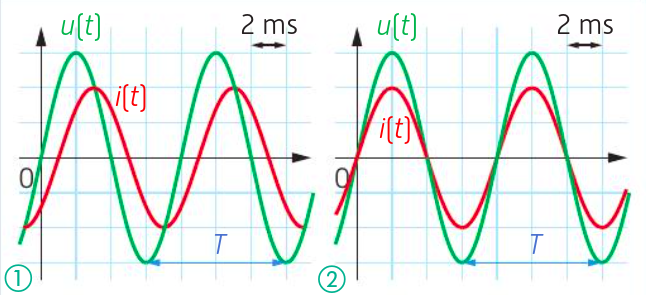
\includegraphics[width=\textwidth]{images/Activite.png}
    \end{minipage}%
    
    
\end{itemize}

\vfill 

\newpage

\noindent%
\begin{minipage}{.42\textwidth}%

    
 \begin{bclogo}[couleur=white!30 ,  arrondi =0.1 , logo = \bcinfo, epBarre =2]{ Matériel }

\begin{itemize*}
    \item 1 GBF
    \item 1 bobine 70mH (0,07 H). 
    \item 1 plaque de test 
    \item 1 multimètre
    \item 1 résistor de 330 $\mathrm{\Omega}$
\end{itemize*}
\end{bclogo}

\end{minipage}%
\hfill
\begin{minipage}{.52\textwidth}%

\begin{circuitikz}

\draw (0,0) to [rmeter, t=GBF] (0,4)--(-2,4); 
\draw (-2,0) to [rmeter, t=V] (-2,4); 
\draw (-2,0)--(4,0) to [R] (4,1.5) to [L]  (4,4) -- (0,4);
\draw (4,0) node[eground]{};
\draw(4,1.8) to [short, o-] (5,1.8) [->] node[right]{Y2};
\draw(4,4) to [short, o-] (5,4) [->] node[right]{Y1};
\end{circuitikz}

\end{minipage}%

\vfill 

\fcolorbox{black}{white}{\textbf{1. Visualisation du déphasage entre u et i dans une bobine}} \\[3mm]


\fcolorbox{black}{white}{\textbf{Montage}}
\begin{itemize*}
    \item Réaliser le montage schématisé ci-dessus \textbf{(L = 0,07 H)}
    \item Réglages préliminaires : 
    \begin{itemize*}
        \item Régler $\mathrm{U=6V}$ et $f\mathrm{=1 000 Hz}$
        \item Régler l'oscilloscope afin de visualiser une période sur l'écran avec l'amplitude la plus grande. 
    \end{itemize*}
    \end{itemize*}
    \defbox{\fbox{
\begin{minipage}{10cm}{

Appel $\mathrm{n^\circ 1}$ - Appeler M Ruiz pour qu'il vérifie le montage.}

\end{minipage}
}}

\vfill 



 

\noindent%
\begin{minipage}{.48\textwidth}%
   \fcolorbox{black}{white}{\textbf{Visualisation}}\\

   
 \begin{bclogo}[couleur=white,  arrondi =0.1 , logo = \bcinfo, epBarre =2]{ Relever l'oscillogramme }

\begin{itemize*}
    \item \textbf{Voie 1 : } On visualise la tension u aux bornes de la bobine. 
    \vspace{3mm}
    \item \textbf{Voie 2 : }On visualise la tension aux bornes de R (on a ainsi une image du
courant i qui traverse la bobine).
\end{itemize*}
\end{bclogo}


\end{minipage}%
\hfill
\begin{minipage}{.45\linewidth}%
 \ecranoscillo
%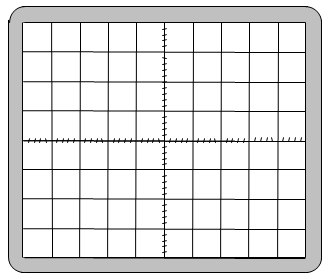
\includegraphics[width=\textwidth]{../Chapitre 2 - Transporter l'énergie sous forme électrique/images/ecran oscillo.png}
\end{minipage}%

\vfill 

\fcolorbox{black}{white}{\textbf{Calcul du déphasage \Large{{$\mathrm{\varphi}$}} 
\normalsize 
entre u (voie 1) et i (voie 2) :}}\\[5mm]

\begin{itemize*}
    \item Relever le décalage $\Delta t$ (en s) entre les deux courbes puis déterminer \Large{$\mathrm{\varphi}$} \normalsize à l'aide de la formule : \\[5mm]

\begin{center}
    \LARGE{$\mathrm{\varphi} = \dfrac{360 \times \Delta t}{T}=$  }
\end{center}
\normalsize
   \item Préciser quelle tension est en avance sur l’autre : \\[5mm]

   \dotfill 

   \item Le déphasage théorique avec une bobine dite parfaite des de 90$^{\circ}$, proposer une explication de l'écart entre la valeur déterminée expérimentalement et la valeur théorique : \\[8mm]

   \dotfill 
   
   
\end{itemize*}

\vfill 



\end{document}